\chapter{Solving Linear Equations}

We have discussed general methods for solving arbitrary equations. For the most part, we restricted our attention to the one-dimensional case. We also looked at a special class of equations, namely those given by polynomials. Another special class is given by linear equations. Of course, the one-dimensional case is absolutely trivial, so one naturally considers systems of equations. 

I assume that you are familiar with the basic results of linear algebra, such as the diagonalization theorems and Gaussian Elimination. This section provides a very quick review, then discusses Singular Value Decomposition (SVD).

\medskip
\noindent \textbf{Applications}: Applications for linear equations are numerous. These include, of course, Linear Programming problems. Other are the local solution of non-linear differential equations via linearization, and the determination of minima in least-squares problems. 

\newpage

\section{A quick review of important definitions and facts}

\begin{enumerate}
\item Given a linear function $f: \mathbb{R}^n \rightarrow \mathbb{R}^m$ and a pair of bases,
    \begin{align*}
        \mathcal{B}_1 &= {e_1,\dots, e_n}\text{ for }\mathbb{R}^n \\
        \mathcal{B}_2 &= {d_1,\dots, d_m}\text{ for }\mathbb{R}^m
    \end{align*}
    we can represent $f$ by an $m\times n$ matrix $A$.

    Notice that the matrix $A$ depends on the choice of bases $\mathcal{B}_1 \times \mathcal{B}_2$.
    
    Often we just let $\mathcal{B}_1 \times \mathcal{B}_2$ be the "obvious" bases for $\mathbb{R}^n \times \mathbb{R}^m$.
    
    \textbf{Moral:} A matrix is a particular coordinate representation of the linear function $f$.
    
\item Given an $m \times n$ matrix $A$, we make the following definitions:
    \begin{align*}
        \text{Column space: } & \text{linear combinations of the columns of }A\\
        \text{Row space: } & \text{linear combinations of the rows of }A
    \end{align*}
    If we think of $A$ as defining the linear mapping 
    \begin{align*}
        A: &\mathbb{R}^n \rightarrow \mathbb{R}^m \\
        &
        \begin{bmatrix} x_1 \\ \vdots \\ x_n \end{bmatrix}
        \rightarrow
        \begin{bmatrix} y_1 \\ \vdots \\ y_m \end{bmatrix}
        =
        A
        \begin{bmatrix} x_1 \\ \vdots \\ x_n \end{bmatrix}
    \end{align*}
    then the column space of $A$ is a vector subspace of $\mathbb{R}^m$, consisting of all points in $\mathbb{R}^m$ that are image vectors under $A$.
    
    Note that the row space of $A$ is just the column space of $A^T$, the transpose of $A$.
    
    And we define
        \begin{align*}
            \text{null space: } & \text{set of vectors }x\text{ in }\mathbb{R}^n\text{ such that }Ax=0.
        \end{align*}
    The following relationships are useful to remember:
    \begin{itemize}
        \item $\dim(\text{row space}) = \dim(\text{column space})$, either of which is called the \underline{rank} of $A$,
        \item The row space and null space are complementary (perpendicular) subspaces of $\mathbb{R}^n$. In other words, 
        \begin{align*}
            \mathbb{R}^n &= \text{row space}\oplus\text{null space} \\
            n &= \dim(\text{row space}) + \dim(\text{null space})
        \end{align*}
    \end{itemize}
    In picture form:
    \begin{figure}[H]
        \centering
        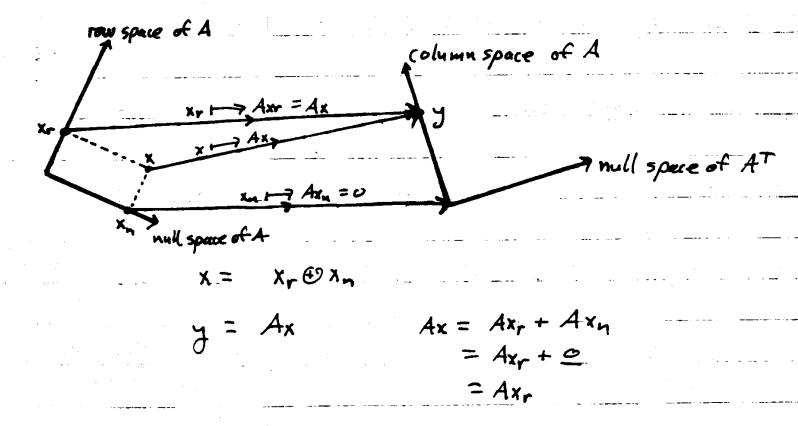
\includegraphics[width=0.9\textwidth]{figures/linear-1.png}
        % \caption{Caption}
        \label{fig:linear-1}
    \end{figure}
    
\item Suppose $A$ is an $m\times n$ matrix, and consider the system of equations 
    \begin{align*}
        Ax = b.
    \end{align*}
    \begin{itemize}
        \item If $b$ is not an element of the column space of $A$, then we say that the system is \underline{inconsistent}(or \underline{overdetermined}). 
        \item If $b$ is in the column space of $A$ and the null space of $A$ is non-trivial, then we say that the system is \underline{underdetermined}. In this case there is a whole family of solutions, given by the affine set
            $$x_0 + N$$
        where $x_0$ is any particular solution $Ax_0 = b$, and $N$ is the null space of $A$. 
        \item If $A$ is a $n\times n$ square matrix we say that $A$ is \underline{singular}
            \begin{description}
                \item \quad iff $\det(A) = 0$
                \item \quad iff $\text{rank}(A) < n$
                \item \quad iff the rows of $A$ are not linearly independent
                \item \quad iff the columns of $A$ are not linearly independent
                \item \quad iff the dimension of the null space of $A$ is non-zero
                \item \quad iff A is not invertible.
            \end{description}
    \end{itemize}
\end{enumerate}

\newpage
\section{Quick review of matrix decompositions}
(we will look at SVD in more detail)

\subsection{Factorizations based on elimination}

Given an $m\times n$ matrix $A$ (with $m \geq n = \text{rank}(A)$), we can write $A$ in the form 
\begin{align*}
    PA &= LDU
\end{align*}
where 
\begin{description}
    \item \quad $P$ is an $m\times m$ permutation matrix that specifies row interchanges, 
    \item \quad $L$ is an $m\times m$ square low-triangular matrix with 1's on the diagonal, 
    \item \quad $U$ is an $m\times n$ upper-triangular matrix with 1's on the diagonal, and 
    \item \quad $D$ is an $m\times m$ square diagonal matrix.
\end{description}

[More generally: we may also need to perform column interchanges on $A$, in which case we get two permutation matrices, so $P_1AP_2 = LDU$.]

Notes:
\begin{enumerate}
    \item The entries on the diagonal of $D$ are sometimes called ``pivots" (after the Gaussian Elimination algorithm). 
    \item The product of the pivots is equal to $\pm\det(A)$ (sign depends on $P$; negative if odd row interchanges), whenever $A$ is a square matrix.
    \item If $A$ is symmetric and $P=I$, then $U=L^T$.
    \item If $A$ is symmetric positive-definite, then $U=L^T$ and the diagonal entries of $D$ are strictly positive.
\end{enumerate}

\underline{Ex}
\begin{enumerate}[label=(a)]
\item 
    \begin{align*}
        \begin{bmatrix}
            1 & 0 \\
            1 & 1 \\
            0 & -1
        \end{bmatrix}
        &=
        \begin{bmatrix}
            1 & 0 & 0 \\
            1 & 1 & 0 \\
            0 & -1 & 1
        \end{bmatrix}
        \begin{bmatrix}
            1 & 0 & 0 \\
            0 & 1 & 0 \\
            0 & 0 & 1
        \end{bmatrix}
        \begin{bmatrix}
            1 & 0 \\
            0 & 1 \\
            0 & 0
        \end{bmatrix}
    \end{align*}
    
    Note: can use any value in the last entry of $D$. Use $0$ if we want $\text{rank}(D) = \text{rank}(A)$.
    
    [If $m > n$, as in this example, then the last $m-n$ rows of $U$ are zero.]

\item
        \begin{align*}
        \begin{bmatrix}
            1 & 1 & 0 \\
            2 & 1 & -1 \\
        \end{bmatrix}
        &=
        \begin{bmatrix}
            1 & 0 \\
            2 & 1
        \end{bmatrix}
        \begin{bmatrix}
            1 & 0 \\
            0 & -1 
        \end{bmatrix}
        \begin{bmatrix}
            1 & 1 & 0 \\
            0 & 1 & 1
        \end{bmatrix}
    \end{align*}
\end{enumerate}

\noindent \underline{Algorithm:} Gaussian Elimination directly yields this decomposition.

\medskip

\noindent \underline{Application:} As with most decompositions/factorizations, the hope is to simplify solving the system $Ax=b$. 

Suppose $A$ is square and non-singular. THen solving $Ax=b$ really means solving 
\begin{align*}
    LDUx &= Pb.
\end{align*}
In turn this entails solving two simpler problems: 
\begin{align*}
    &\text{(i) } Ly = Pb & \text{(solve for $y$)} \\
    &\text{(ii) } Ux = D^{-1}y & \text{(solve for $x$)}
\end{align*}
Each of these problems can be solved easily using forward or back substitution ($D^{-1}$ is easy to compute since $0$ is diagonal with non-zero entries).

\subsection{Factorizations based on eigenvalues}

These are the standard factorization s one learns in a linear algebra course. Two important ones are:

\begin{enumerate}
\item If $A$ is a square $n\times n$ matrix with $n$ linearly independent eigenvectors, then
    \begin{align*}
        A &= S\Lambda S^{-1},
    \end{align*}
    where $\Lambda$ is a diagonal matrix whose entries are the eigenvalues of $A$,
    
    \medskip
    
    and $S$ is a matrix whose columns are the eigenvectors of $A$.
    
    \medskip
    
    This factorization is not always possible. (One case in which it is possible ofccurs when $A$ has $n$ distinct eigenvalues.)

\item One can always decompose $A$ in Jordan form, i.e.,
    \begin{align*}
        A &= MJM^{-1}
    \end{align*}
    where $J = 
    \begin{bmatrix}
        J_1 & \dots & 0 \\
        \vdots & \ddots & \vdots \\
        0 & \dots & J_s
    \end{bmatrix}
    $ is a block matrix, such that each block \newline
    $J_i = 
    \begin{bmatrix}
        \lambda_i^1 & \dots & 0 \\
        \vdots & \ddots & \vdots \\
        0 & \dots & \lambda_i^s
    \end{bmatrix}
    $ with $\lambda_i$ an eigenvalue of $A$.

    \medskip
    
    Here $s$ is the number of independent eigenvectors of $A$. $M$ consists of eigenvectors and ``generalized" eigenvectors.

    \medskip
    
    [Side note: ]

\end{enumerate}

\subsection{Factorizations based on $A^TA$}

\subsubsection{QR}

\subsubsection{SVD}

\subsection{SVD in more detail}